\documentclass[titlepage,a4paper]{jsarticle}
\usepackage{../../sty/import}% 各種パッケージインポート
\usepackage{../../sty/title_kyoudou}% タイトルページの変更

%% タイトルページの変数
% レポートタイトル
\title{量子コンピュータプログラミング}
% 提出日
\expdate{\today}
% 科目名
\subject{情報システム工学実験}
% 分野
\class{情報経営システム工学分野}
% 学年
\grade{B3}
% 学籍番号
\mynumber{24336488}
% 記述者
\author{本間三暉}
% グループ名 % もし班があるやつならtitle_team.styを入れる
\coauthor{%
{学籍番号:}22100289 & {氏名:}浅野 繭\\
{学籍番号:}22105590 & {氏名:}筒井 翼\\
{学籍番号:}22100986 & {氏名:}板山修大\\
}
%
%記載例:
%\coauthor{%
%  2番 & 新潟 花子\\
%  11番 & 三条 次郎}
%%
\begin{document}
% titleページ作成
\maketitle
\section{目的}
% ・今回の実験について,自分なりに設定した目的を記述して下さい.
この実験の目的は,量子コンピュータの基本原理とプログラミング技術を習得することにある.
この実験では,量子ビット(キュービット)の基礎概念や,重ね合わせ,もつれといった量子特有の性質を理解し,古典的なビットとの違いを明確にする.
また,基本的な量子ゲート(Hadamardゲート,Pauliゲート,CNOTゲートなど)の操作方法を学び,これらを用いた量子回路の設計と実装の方法を習得することを目指す.
さらに,ショアのアルゴリズムやグローバーのアルゴリズムなどの代表的な量子アルゴリズムを理解し,これらを実際にプログラムとして実装する.

プログラミングの実践においては,QiskitやCirqなどの量子コンピュータプログラミングフレームワークを用いたプログラミングスキルを習得し,実際の量子コンピュータ上でプログラムを実行する経験を得ることを目的とする.
これにより,量子計算が解決できる問題の種類や応用分野についても検討し,従来のコンピュータでは実現困難な計算の可能性を理解する.

この実験を通じて,参加者は量子コンピュータの基礎から応用までの広範な知識を習得し,将来的に量子技術の研究や実務に貢献できる能力を身につけることを目指す.
\section{原理}
% ・量子論理回路,グローバーのアルゴリズムについて説明してください.
\subsection{量子論理回路}
\subsection*{概要}
量子論理回路は,量子ビット(キュービット)を操作するための基本単位である.
従来の論理回路が古典ビットを用いるのに対し,量子論理回路は量子力学の原理に基づいて動作する.
これにより,並列処理能力や量子重ね合わせ,量子もつれといった特性を活用することが可能である.

\subsection*{量子ビット}
量子ビットは,0と1の状態を同時にとることができる量子重ね合わせの性質を持つ.
これは,$|0\rangle$ と$|1\rangle$ の状態の重ね合わせとして表現される.量子ビットの状態は式\eqref{psii}のように表される.
\begin{align}
  |\,\psi \rangle & = \alpha|\,0\rangle + \beta|\,1\rangle \label{psii}
\end{align}
ここで,$\alpha$と$\beta$は複素数であり,$|\alpha|^2+|\beta|^2=1$である.
\subsection*{量子ゲート}
量子論理回路は,量子ゲートと呼ばれる基本的な演算を組み合わせて構成される.
代表的な量子ゲートには以下のようなものがある.
\subsubsection*{Hadamardゲート(Hゲート)}
量子ビットを重ね合わせ状態に変換する.
\begin{align}
  H|\,0\rangle & = \frac{1}{\sqrt{2}}\left(|\,0\rangle + | \, 1 \rangle\right) \\
  H|\,1\rangle & = \frac{1}{\sqrt{2}}\left(|\,0\rangle - | \, 1 \rangle\right)
\end{align}
\subsubsection*{Pauli-Xゲート}
古典論理回路のNOTゲートに相当する.
\begin{align}
  X|\,0\rangle & = X|\,1\rangle \\
  X|\,1\rangle & = X|\,0\rangle
\end{align}
\subsubsection*{CNOTゲート (制御NOTゲート)}
2量子ビットゲートで,制御ビットが1のときにターゲットビットを反転させる.
\begin{align}
  CNOT(|a\rangle \otimes |b\rangle) & = |a\rangle \otimes(a \oplus b)
\end{align}

\subsection*{量子回路の設計}
量子回路は,量子ビットを初期化し,量子ゲートを適用して計算を行い,最終的に測定するという一連のステップで設計される.
これにより,量子ビットの状態を古典ビットに変換し,結果を得ることができる.
\subsection{グローバーのアルゴリズム}
グローバーのアルゴリズムは,無条件検索問題(非構造的データベースの検索)に対する量子アルゴリズムである.
古典的なアルゴリズムでは$O(N)$の時間がかかる検索問題を,グローバーのアルゴリズムでは$O(\sqrt{N})$の時間で解くことができる.
\subsubsection*{アルゴリズムのステップ}
\subsubsection{初期化}
すべての量子ビットを$|\,0\rangle$に初期化し,Hadamardゲートを適用してすべての状態の重ね合わせを生成する.
\begin{align}
  H^{\otimes n}|0\rangle = \frac{1}{\sqrt{N}} \sum_{x=0}^{N-1} |x\rangle
\end{align}
\subsubsection{オラクル(Oracle)の適用}
オラクルは,解となる状態を反転させる役割を果たす.状態$|\,x\rangle$が解である場合,$-1$の位相が付加される.
\begin{align}
  U_f|x\rangle = (-1)^{f(x)}|x\rangle
\end{align}
\subsubsection{拡散変換(Amplitude Amplification)}
拡散変換は,解の確率振幅を増幅させる操作である.これは,状態ベクトル全体を平均値に対して反転させることによって実現される.
\begin{align}
  U_s = 2|\,\psi\rangle \langle \psi\,| - I
\end{align}
\subsubsection{反復}
オラクルと拡散変換を$\sqrt{N}$回繰り返すことで,解の確率振幅を最大化する.
\subsubsection{測定}
最後に量子ビットを測定することで,高確率で解が得られる.

\section{論理パズル}\label{パズル}
% ・グループで考えた論理パズル2人用,3人用,4人用
% についてわかりやすく記述してください.
% ・自分の担当部分を明記してください.
グループメンバー全員で相談して決めたので,誰がどこをやるかみたいな明確な割振りはしていません.
\subsection{2人用}
殺人事件が起きました.容疑者は二人おり,それぞれ次のように述べています.
\begin{itemize}
  \item [エリカ]「アリスが犯人です」
  \item [アリス]「私たちのどちらも犯人です」
\end{itemize}
犯人は一人です.
一人が本当のことを言っていますが,もう一人は嘘をついています.
犯人は誰でしょう.

\subsection{3人用}
コナン君の目の前で歩美ちゃん,元太君,光彦君が突然次のようなことを述べ始めました.
\begin{itemize}
  \item [歩美]「元太君は黒幕じゃないよ」
  \item [元太]「俺は黒幕じゃない」
  \item [光彦]「元太君は黒幕です」
\end{itemize}
黒幕を特定してください.

\subsection{4人用}
黒の組織でスパイが紛れ込んでいることが分かりました.そこで,スパイ疑惑をかけられているキール,ジン,ライ,バーボンは次のように主張しています.
\begin{itemize}
  \item [キール]「ライがスパイよ」
  \item [ジン]「俺はスパイじゃねぇ」
  \item [ライ]「バーボンはスパイだ」
  \item [バーボン]「ライはうそつきだ」
\end{itemize}
彼らのうち3人が嘘をついています.スパイを特定してください.
\section{パズルの論理式}
% ・グループで考えたパズルの論理式についてわかりやすく記述してください.
% ・自分の担当部分を明記してください.
節\ref{パズル}と同様に,グループメンバー全員で相談しながら考えたので,明確な割振りはしていません.
基本的に犯人である事象を$X$,嘘をついている事象を$Y$とする.
\subsection{2人用}
\begin{tabular}[t]{l@{\hspace{0.5\zw}:\hspace{0.5\zw}}l}
  エリカが犯人である & $X_1$ \\
  アリスが犯人である & $X_2$ \\
  エリカが正直である & $Y_1$ \\
  アリスが正直である & $Y_2$ \\
\end{tabular}

\begin{tabular}[t]{rl@{:\hspace{0.5\zw}}l}
  エリカ & 「犯人はアリスである」 & $Y_1 \cdot X_2 \cdot (\overline{\overline{Y_1}} \cdot \overline{\overline{X_2}}) = Y_1 \cdot X_2$ \\
  アリス & 「二人とも犯人である」 & $Y_1 \cdot (X_1 \cdot X_2) \cdot \overline{X_2} = X_1 \cdot Y_1 \cdot \phi$(恒偽命題)                 \\
\end{tabular}
\subsection{3人用}
\begin{tabular}[t]{l@{\hspace{0.5\zw}:\hspace{0.5\zw}}l}
  歩美が黒幕である & $X_1$ \\
  元太が黒幕である & $X_2$ \\
  光彦が黒幕である & $X_3$ \\
  歩美が正直である & $Y_1$ \\
  元太が正直である & $Y_2$ \\
  光彦が正直である & $Y_3$ \\
\end{tabular}

\begin{tabular}[t]{rl@{:\hspace{0.5\zw}}l}
  歩美 & 「元太君は黒幕ではない」 & $Y_1 \cdot \overline{X_2} \cdot \overline{\overline{X_2}} \cdot \overline{X_2} = Y_2 \cdot \phi$(恒偽命題) \\
  元太 & 「俺は黒幕じゃない」   & $Y_2 \cdot \overline{X_2} \cdot \overline{\overline{X_2}} = Y_2 \cdot \phi$(恒偽命題)                      \\
  光彦 & 「元太君は黒幕である」  & $Y_3 \cdot X_2 \cdot \overline{\overline{X_2}} = Y_3 \cdot X_2$                                        \\
\end{tabular}
\subsection{4人用}
\begin{tabular}[t]{l@{\hspace{0.5\zw}:\hspace{0.5\zw}}l}
  キールがスパイである  & $X_1$ \\
  ジンがスパイである   & $X_2$ \\
  ライがスパイである   & $X_3$ \\
  バーボンがスパイである & $X_4$ \\
  キールが正直である   & $Y_1$ \\
  ジンが正直である    & $Y_2$ \\
  ライが正直である    & $Y_3$ \\
  バーボンが正直である  & $Y_4$ \\
\end{tabular}

\begin{tabular}[t]{rl@{:\hspace{0.5\zw}}l}
  キール  & 「ライがスパイよ」   & $Y_1 \cdot X_3 \cdot \overline{\overline{X_2}} \cdot\overline{X_4} \cdot \overline{\overline{Y_3}}$  \\
  ジン   & 「俺はスパイじゃねぇ」 & $Y_2 \cdot \overline{X_2} \cdot \overline{X_3} \cdot \overline{X_4} \cdot \overline{\overline{Y_3}}$ \\
  ライ   & 「バーボンはスパイ」  & $Y_3 \cdot X_4 \cdot \overline{X_3} \cdot \overline{\overline{X_2}} \cdot \overline{\overline{Y_3}}$ \\
  バーボン & 「ライは嘘つきさ」   & $Y_4 \cdot \overline{Y_3} \cdot \overline{X_3} \cdot \overline{\overline{X_2}} \cdot \overline{X_4}$ \\
\end{tabular}

\section{量子回路}
% ・パズルを解く回路を記載し,その回路について説明してください.
% ・自分の担当部分を明記してください.
2人,3人及び,4人の場合の論理パズルを解く量子論理回路について説明を行う.
\subsection{2人用}
2人用の論理パズルの真理値表を表\ref{2:真理値}に,量子論理回路を図\ref{2:回路}に,ソースコードをソースコード\ref{2:ソースコード}に示す.
\begin{table}[H]
  \centering
  \caption{2人用真理値表}
  \label{2:真理値}
  % tabler環境の挿入
  \begin{tabular}{lll|lll}
                                                  &     & \multicolumn{2}{c|}{犯人は?} & \multicolumn{2}{c}{正直者は?}             \\\hline
                                                  &     & エリカ                       & アリス                       & エリカ & アリス \\
    \multicolumn{1}{c}{\multirow{2}{*}{誰の証言が正しい}} & エリカ &                           & 〇                         & 〇   &     \\
    \multicolumn{1}{c}{}                          & アリス & 〇                         & 〇                         &     & 〇
  \end{tabular}
\end{table}

\begin{figure}[H]
  \centering
  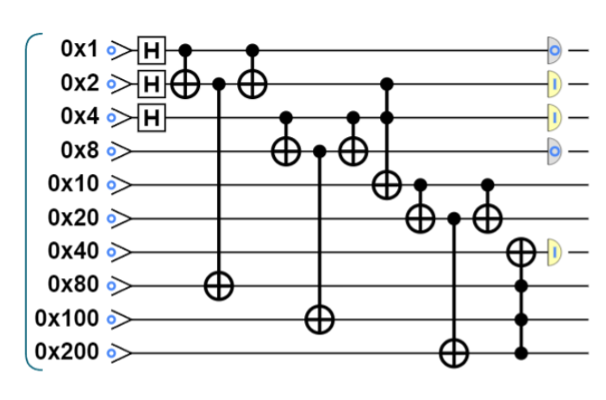
\includegraphics[width=0.8\textwidth]{img/2_qc.png}
  \caption{2人用量子論理回路}
  \label{2:回路}
\end{figure}

\begin{lstlisting}[caption=2人用QCEngin,label=2:ソースコード]
  qc.reset(10);         
  qc.write(0b0000000000);         
  \\ 定義
  var x1=0x1;
  var x2=0x2;
  var y1=0x4;
  var y2=0x8;
  var comment1=0x10;
  var comment2=0x20;
  var result=0x40;
  var x1_xor_x2=0x80;
  var y1_xor_y2=0x100;
  var comment1_xor_comment2=0x200;
  
  qc.had(x1|x2|y1);

  xor2(x1,x2,x1_xor_x2);

  xor2(y1,y2,y1_xor_y2);

  and2(y1,x2,comment1);

  xor2(comment1,comment2,comment1_xor_comment2);
  
  qc.cnot(result,x1_xor_x2|y1_xor_y2|comment1_xor_comment2);
 
  qc.read(x1|x2|y1|y2|result);

  \\--------------------------
  \\ 関数
  \\--------------------------
  function and2(x,y,result){
      qc.cnot(result,x|y);
  }
  
  function or2(x,y,result){
      qc.not(x|y);
      qc.cnot(result,x|y);
      qc.not(x|y|result);
  }
  
  function xor2(x,y,result){
      qc.cnot(y,x);
      qc.cnot(result,y);
      qc.cnot(y,x);
  }
\end{lstlisting}
まず,量子コンピュータの10量子ビットをリセットし,すべての量子ビットを初期状態(0)に設定する.
各変数は異なる量子ビットを表しており,x1やx2などがそれに該当する.
次に,x1,x2,y1のビットにアダマール変換を適用し,これらのビットを重ね合わせ状態にする.
ただし,y2については,問題の設定上アリスが正直であることがないため,アダマール変換は適用しなかった.

続いて,x1とx2のXOR結果をx1\_xor\_x2に,y1とy2のXOR結果をy1\_xor\_y2に保存する.
これは,それぞれ犯人が一人であることと正直者が一人であることを示している.
次に,y1とx2のAND結果をcomment1に保存し,エリカの証言「アリスが犯人です」を適応する.
さらに,エリカの証言とアリスの証言のXOR結果をcomment1\_xor\_comment2に保存し,アリスの証言「私たちのどちらも犯人です」を適応する.

次に,XORされた証言の結果が嘘であることを示すためにresultに保存する.
最後に,x1,x2,y1,y2,およびresultのビットを読み取り,最終結果を得る.
このようにして,特定の条件を満たすかどうかを検証し,エリカとアリスの証言の整合性を確認し,犯人を判定する.

\subsection{3人用}
人用の論理パズルの真理値表を表\ref{3:真理値}に,量子論理回路を図\ref{3:回路}に,ソースコードをソースコード\ref{3:ソースコード}に示す.
\begin{table}[H]
  \centering
  \caption{3人用真理値表}
  \label{3:真理値}
  % tabler環境の挿入
  \begin{tabular}{c|l|lll|lll}
    \multicolumn{1}{l}{}      &      & \multicolumn{3}{c|}{黒幕は?} & \multicolumn{3}{c}{正直者は?}                           \\\hline
    \multicolumn{1}{l}{}      &      & あゆみ                       & げんた                       & みつひこ & あゆみ & げんた & みつひこ \\\hline
    \multirow{3}{*}{誰の証言が正しい} & あゆみ  &                           & ×                         &      & 〇   & ×   & 〇    \\
                              & げんた  &                           & ×                         &      & ×   & 〇   & 〇    \\
                              & みつひこ &                           & 〇                         &      & ×   & ×   & 〇    \\\hline
  \end{tabular}
\end{table}

\begin{figure}[H]
  \centering
  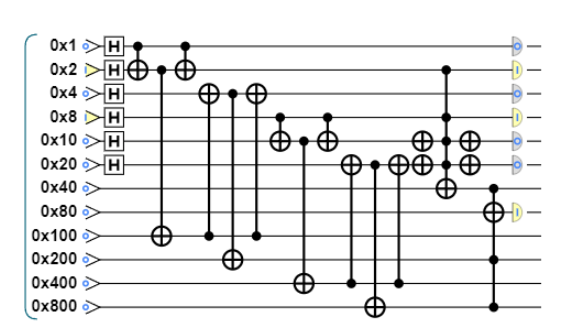
\includegraphics[width=0.8\textwidth]{img/3_qc.png}
  \caption{3人用量子論理回路}
  \label{3:回路}
\end{figure}

\begin{lstlisting}[caption=3人用QCEngin,label=3:ソースコード]
  qc.reset(12);         
  qc.write(0b0000001010);         
  
  var x1=0x1;
  var x2=0x2;
  var x3=0x4;
  var y1=0x8;
  var y2=0x10;
  var y3=0x20;
  var comment=0x40;
  var result=0x80;
  var x1_xor_x2=0x100;
  var x12_xor_x3=0x200;
  var y1_xor_y2=0x400;
  var y12_xor_y3=0x800;
  
  
  qc.had(x1|x2|x3|y1|y2|y3);
  
  xor2(x1,x2,x1_xor_x2);
  xor2(x1_xor_x2,x3,x12_xor_x3);
  xor2(y1,y2,y1_xor_y2);
  xor2(y1_xor_y2,y3,y12_xor_y3);
  
  qc.not(y2|y3);
  qc.cnot(comment,y1|x2|y2|y3);
  qc.not(y2|y3);
  
  qc.cnot(result,x12_xor_x3|y12_xor_y3|comment);
  qc.read(x1|x2|x3|y1|y2|y3|result);
  
  function and2(x,y,result){
      qc.cnot(result,x|y);
  }
  
  function or2(x,y,result){
      qc.not(x|y);
      qc.cnot(result,x|y);
      qc.not(x|y|result);
  }
  
  function xor2(x,y,result){
      qc.cnot(y,x);
      qc.cnot(result,y);
      qc.cnot(y,x);
  }
\end{lstlisting}
まず,量子コンピュータの12量子ビットを初期化し,特定のビット(2番目と4番目)を1に設定する.
これにより,初期状態がセットされる.
各変数は異なる量子ビットを表しており,x1やx2などがそれに対応する.
次に,x1,x2,x3,y1,y2,y3のビットにアダマール変換を適用して,これらのビットを重ね合わせ状態にする.
続いて,x1とx2のXOR結果をx1\_xor\_x2に,x1\_xor\_x2とx3のXOR結果をx12\_xor\_x3に保存することで特定の条件を表現し,y1とy2のXOR結果をy1\_xor\_y2に,y1\&\_xor\_\&y2とy3のXOR結果をy12\_xor\_y3に保存することで別の条件を表現する.
さらに,y2とy3のビットを反転させ,反転させたy2とy3を含めたAND結果をcommentに保存し,再度y2とy3のビットを元に戻す.
そして,XORされた結果とcommentを組み合わせ,その結果をresultに保存することで特定の条件が満たされていることを示し,最後にx1,x2,x3,y1,y2,y3,およびresultのビットを読み取り最終結果を得る.
また,AND,OR,XORの操作を行う関数を定義し,and2はxとyのAND結果をresultに,or2はxとyのOR結果をresultに,xor2はxとyのXOR結果をresultに保存する.
このようにして,特定の条件を検証するために量子ビットを操作し,設定された条件の下で証言の整合性を確認し,特定の結論に達する.
\subsection{4人用}
4人用の論理パズルの真理値表を表\ref{4:真理値}に,量子論理回路を図\ref{4:回路}に,ソースコードをソースコード\ref{4:ソースコード}に示す.
\begin{table}[H]
  \centering
  \caption{4人用真理値表}
  \label{4:真理値}
  % tabler環境の挿入
  \begin{tabular}{c|l|llll|llll}
    \multicolumn{1}{l}{} &      & \multicolumn{4}{c|}{スパイは?} & \multicolumn{4}{c}{正直者は?}                                     \\\hline
    \multicolumn{1}{l}{} &      & ジン                         & ライ                        & バーボン & キール & ジン & ライ & バーボン & キール \\\hline
    \multirow{2}{*}{証言の} & ジン   & ×                          & ×                         & 〇×   &     & 〇  & 〇  &      &     \\
    \multirow{2}{*}{正しさ} & ライ   & 〇                          & ×                         & 〇    &     &    & 〇  &      &     \\
                         & バーボン & 〇                          & ×                         & ×    &     &    & ×  & 〇    &     \\
                         & キール  & 〇                          & 〇                         & ×    &     &    & 〇  &      & 〇   \\\hline
  \end{tabular}
\end{table}

\begin{figure}[H]
  \centering
  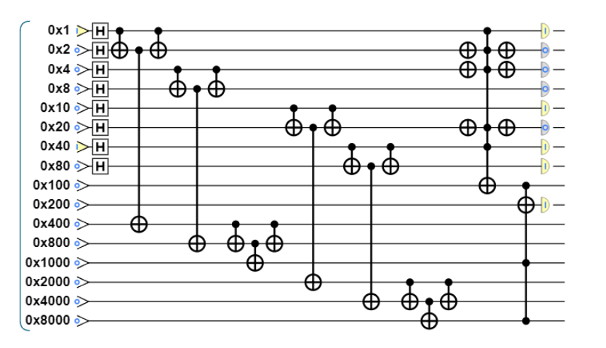
\includegraphics[width=0.8\textwidth]{img/4_qc.png}
  \caption{4人用量子論理回路}
  \label{4:回路}
\end{figure}

\begin{lstlisting}[caption=2人用QCEngin,label=4:ソースコード]
  qc.reset(16);         
qc.write(0b0000000001000001);         

var x1=0x1;
var x2=0x2;
var x3=0x4;
var x4=0x8;
var y1=0x10;
var y2=0x20;
var y3=0x40;
var y4=0x80;
var comment=0x100;
var result=0x200;
var x1_xor_x2=0x400;
var x3_xor_x4=0x800;
var x12_xor_x34=0x1000;
var y1_xor_y2=0x2000;
var y3_xor_y4=0x4000;
var y12_xor_y34=0x8000;

qc.had(x1|x2|x3|x4|y1|y2|y3|y4);

xor2(x1,x2,x1_xor_x2);
xor2(x3,x4,x3_xor_x4);
xor2(x1_xor_x2,x3_xor_x4,x12_xor_x34);
xor2(y1,y2,y1_xor_y2);
xor2(y3,y4,y3_xor_y4);
xor2(y1_xor_y2,y3_xor_y4,y12_xor_y34);

qc.not(x2|x3|y2);
qc.cnot(comment,y3|x2|y2|x3|x1);
qc.not(x2|x3|y2);

qc.cnot(result,x12_xor_x34|y12_xor_y34|comment);
qc.read(x1|x2|x3|x4|y1|y2|y3|y4|result);

function and2(x,y,result){
    qc.cnot(result,x|y);
}

function or2(x,y,result){
    qc.not(x|y);
    qc.cnot(result,x|y);
    qc.not(x|y|result);
}

function xor2(x,y,result){
    qc.cnot(y,x);
    qc.cnot(result,y);
    qc.cnot(y,x);
}
\end{lstlisting}
最初に,量子コンピュータの16量子ビットをリセットし,特定のビット(最下位ビットと7番目のビット)を1に設定して初期状態を確立する(正解の確認のため).
各変数は異なる量子ビットを表し,x1からx4,およびy1からy4がそれに該当する.
次に,x1,x2,x3,x4,y1,y2,y3,y4のビットにアダマール変換を適用し,それらを重ね合わせ状態にする.

その後,x1とx2のXOR結果をx1\_xor\_x2に,x3とx4のXOR結果をx3\_xor\_x4に保存し,さらにこれらの結果をXORしてx12\_xor\_x34に保存することで,特定の条件を表現する.
同様に,y1とy2のXOR結果をy1\_xor\_y2に,y3とy4のXOR結果をy3\_xor\_y4に保存し,さらにこれらの結果をXORしてy12\_xor\_y34に保存することで,別の条件を示す.

続いて,x2,x3,y2のビットを反転させ,反転させた状態でy3,x2,y2,x3,x1のAND結果をcommentに保存し,再度ビットを反転して元に戻す.
次に,XORされた結果とcommentを組み合わせ,その結果をresultに保存することで特定の条件が満たされていることを示す.
最後に,x1,x2,x3,x4,y1,y2,y3,y4,およびresultのビットから最終結果を得る.

プログラム上で,AND,OR,XORの操作を行う関数も定義されており,and2はxとyのAND結果をresultに,or2はxとyのOR結果をresultに,xor2はxとyのXOR結果をresultに保存する.
このように,特定の条件を検証するために量子ビットを操作し,特定の前提の下で証言の整合性を確認し結論を導き出す.
\section{実行結果}
% ・QCEngine とIBMQ のシミュレータでの結果を掲載してください.
\subsection{2人用}
図\ref{2:circle}に2人用のQCEnginのCircle notationを,図\ref{2:ibmq}に2人用のIBMQで作成したグラフを示す.
\begin{figure}[H]
  \centering
  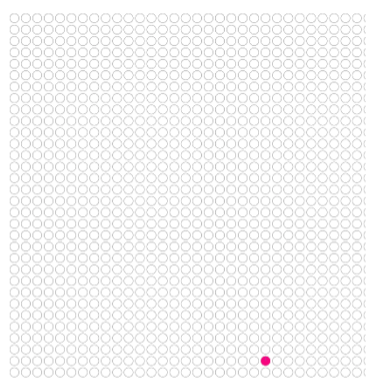
\includegraphics[width=0.8\textwidth]{img/2_circle.png}
  \caption{2人用QCEngin Circle notation}
  \label{2:circle}
\end{figure}
\begin{figure}[H]
  \centering
  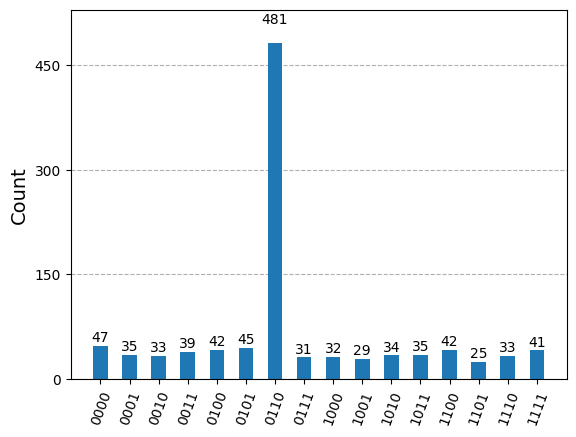
\includegraphics[width=0.8\textwidth]{img/2_kairyou_python.png}
  \caption{2人用IBMQ結果}
  \label{2:ibmq}
\end{figure}

\subsection{3人用}
図\ref{3:circle}に3人用のQCEnginのCircle notationを,図\ref{3:ibmq}に3人用のIBMQで作成したグラフを示す.
\begin{figure}[H]
  \centering
  
\includegraphics[width=0.8\textwidth]{img/3_circle.png}
  \caption{3人用QCEngin Circle notation}
  \label{3:circle}
\end{figure}
\begin{figure}[H]
  \centering
  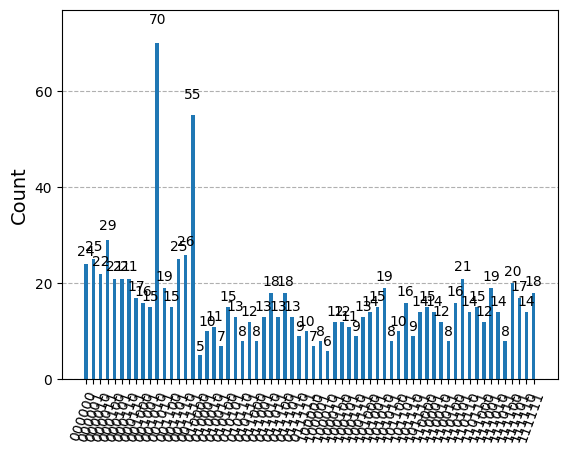
\includegraphics[width=0.8\textwidth]{img/3_kairyou_python.png}
  \caption{3人用IBMQ結果}
  \label{3:ibmq}
\end{figure}

\subsection{4人用}
図\ref{4:circle}に4人用のQCEnginのCircle notationを,図\ref{4:ibmq}に4人用のIBMQで作成したグラフを示す.
\begin{figure}[H]
  \centering
  
\includegraphics[width=0.8\textwidth]{img/4_circle.png}
  \caption{4人用QCEngin Circle notation}
  \label{4:circle}
\end{figure}
\begin{figure}[H]
  \centering
  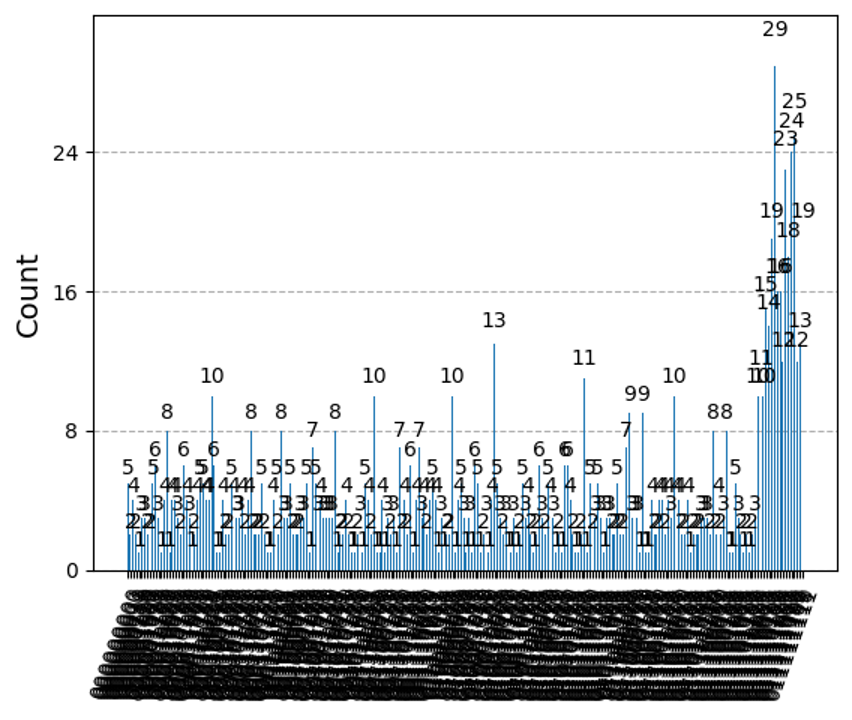
\includegraphics[width=0.8\textwidth]{img/4_kairyoou_python.png}
  \caption{4人用IBMQ結果}
  \label{4:ibmq}
\end{figure}
\section{考察}
% ・実験結果について考察してください.
2人用3人用4人用のすべてでcircle notationは最終的に1つのみ量子ビットが1になった.
これはただ一つの解を持つことにほかならない.
私の班は全ての論理パズルで解が1つは1つなので,論理パズルの解とcircle notationを照らし合わせると結果は正しいと言える.

また,IBMQシミュレーターの結果について考察する.
2人用のパズルでは,図\ref{2:ibmq}に示す通り,0110だけ抜き出ていて,論理パズルの正解の組み合わせと合致するので精度の高い結果になっていると言える.

3人用のパズルでは,図\ref{3:ibmq}に示す通り,正解の値とは別にもう一つ値が抜き出てしまっている.
そのため,論理パズルの内容を正しく論理式に反映できなかった可能性やそもそも論理パズルに複数の解がある可能性,
論理式は正しいがそれをIBMQのソースコードにする過程で間違ってしまった可能性が考えられる.
図\ref{3:circle}に示す通り,circle notationでは解が1つに求まっているので,IBMQのソースコードにする過程で間違ってしまった可能性が高いと考える.
この場合,比較的容易に改善できると考える.

4人用のパズルでは,図\ref{4:ibmq}に示す通り,おおよその解の方向性はわかるが,ここから1つや2つに解を絞ることは難しい事がわかる.
考えられる可能性は3人用のときと同様であるが,図\ref{4:circle}の結果も踏まえると,
3人用のときに比べパズルやその論理式が複雑であるため,IBMQシミュレーターに起こす過程でミスがあったのではないかと考える.
また,今回はIBMQシミュレーターのサンプル数が選択肢に対して多いわけではないため,その分シミュレーション結果が分散してしまった可能性も考えられる.
この場合,サンプル数を増やせば解決するのではないかと考える.

\section{感想}
% ※ここは採点の対象外です.
% 今回の実験の内容について感想などあれば記述して下さい.
% 次年度以降の実験の実施に役立てたいと思います.
レポートを書く際に結果を使ったりするのならば,ソースコードを保存した方が良いなど実験中に言ってくれると嬉しかった.

それはそれとして,実験内容自体は面白かった.
また,高専でやった論理回路の良い復習になったと思う.
\end{document}
